%%%%%%%%%%%%%%%%%%%%%%%[Comments]%%%%%%%%%%%%%%%%%%%%%%%
% Starting from February 2021, SNU students are no longer required to submit a printed dissertation; only a digital version is necessary. Consequently, the library no longer enforces strict rules for page size, margin size, fonts, and font sizes. Their guidance is to "basically follow the template." 
%
% Therefore, most parts in this document are free to be changed, especially within the %%%%[Free to change]%%%% block, as long as it doesn't significantly compromise readability.
%
% ******* If you want the true bare-bone structure, go to ********
% https://github.com/taehoonlee/snu-dissertation-template
%
% """중앙도서관에서 LaTex 양식은 별도로 제공하고 있지 않으며, word / 한글 양식만 제공하고 있는 점 양해 부탁드립니다. [...] 현재 저희가 제공하고 있는 작성 요령 및 내용 구성 등은 기본적으로 따르되, 많이 문의해주시는 논문의 규격(본문 크기, 여백 등), 서체(활자 종류 및 크기)에 대해서는 엄격하게 규정해두고 있지 않은 점 알려드립니다."""  - email by libit@snu.ac.kr on 2022-12-05 to ysBach.
%
% 서울대학교 학위논문 LaTeX 템플릿 (한글 논문) kungmo@snu.ac.kr (2025년 2월)
%%%%%%%%%%%%%%%%%%%%%%%%%%%%%%%%%%%%%%%%%%%%%%%%%%%%%%%%
% !TEX encoding = UTF-8 Unicode

\documentclass[12pt]{report}
\usepackage[paperwidth=21cm,paperheight=29.7cm,left=2.5cm,right=2.5cm,top=3.5cm,bottom=1.5cm]{geometry}
% Originally this was
%\usepackage[paperwidth=19cm,paperheight=26cm,left=3cm,right=3cm,top=3.5cm,bottom=1.5cm]{geometry}

% 국문 논문으로 바꾸려고 추가함 20240521
% 한글 출력 관련 설정
\usepackage[hangul]{kotex}
\usepackage{kotex-logo}
\usepackage{indentfirst}

% 표 관련 설정 20240729
\usepackage{lscape}
\usepackage{tabularx,booktabs,caption,multirow,array}
\usepackage{longtable}
\usepackage[table,xcdraw]{xcolor}
\usepackage{colortbl}

\addtolength{\voffset}{-1.5cm}
\renewcommand{\baselinestretch}{2.0} % 기본 줄간격 1.7
\renewcommand{\abstractname}{\large 국문초록} % Abstract를 '국문초록'으로 20240521
\usepackage{setspace}
\usepackage[]{enumitem}
%\usepackage{lmodern}
%\usepackage{librecaslon}
%\usepackage[T1]{fontenc}
\usepackage{footnote}
\usepackage{textcomp}
\usepackage{verbatim} % comment 처리하려고 추가함 20240521
%%%%%%%%%%%%%%%%%%%%%%%%%%%%%%%%%%%%%%%%%
%% Reference style settings
%% ↓ This is also free to change. Do as you wish...
%\usepackage[
%  round,
%  semicolon,
%  authoryear,
%%  sort
%]{natbib}

%%%%%%% BIB %%%%%%%%%%%%%%%%%
%% KTUG.org의 noname님 감사합니다!! 덕분에 한글 이름과 영어 이름 인용을 자동으로 처리할 수 있게 되었습니다. 20240811
\usepackage[
	backend=biber,
	bibencoding=utf8,
%	style=apa,
	natbib=true,
	citestyle=authoryear,
	bibstyle=authoryear, 
	maxcitenames=2,
	maxbibnames=9,
	language=auto,
	autolang=other,
	uniquelist=false,
	dashed=false
]{biblatex}
\renewcommand\nameyeardelim{, }	%% natbib command. natbib should be true.
\renewbibmacro{in:}{}

\newcommand*{\myownetal}{et~al.}
\newcommand*\MYand{and}
\DefineBibliographyStrings{english}{%
	andothers={\myownetal}{},
	and={\MYand}{}
}

\let\origbibleftparen\bibleftparen
\newcommand*\MYbibleftparen{\origbibleftparen}
\renewcommand*\bibopenparen{\MYbibleftparen}
\renewcommand*\bibcloseparen{\bibrightparen}

\AtEveryCitekey{%
  \ifkeyword{kobib}{%
    \renewcommand{\multinamedelim}{·}%
    \renewcommand{\finalnamedelim}{·}%
    \renewcommand*{\myownetal}{외}%
    \renewcommand*\MYand{\unskip\와}%
    \renewcommand*\MYbibleftparen{\unskip\origbibleftparen}%
  }{}%
}

\AtEveryBibitem{%
  \clearfield{note}%
  \ifkeyword{kobib}{%
    \renewcommand{\multinamedelim}{·}%
    \renewcommand{\finalnamedelim}{·}%
	\renewcommand*\mkbibquote[1]{〈#1\isdot〉}
    \DeclareFieldFormat{journaltitle}{『#1』}%
	\DeclareFieldFormat{title}{『#1』}%
	\DeclareFieldFormat{translator}{#1 (역)}
  }{%
	\renewcommand*\mkbibquote[1]{``#1\isdot''}
	\ifkeyword{kobibmixed}{
		\renewcommand{\multinamedelim}{, }%
		\renewcommand{\finalnamedelim}{, }%
	    \DeclareFieldFormat{journaltitle}{『#1』}%
		\DeclareFieldFormat{title}{『#1』}%
		\DeclareFieldFormat{translator}{#1 (역)}
	}{}	
  }
}%

\addbibresource{references.bib}

%%%%%%%%%%%%%%%%%%%%
% Page numbering style settings
% For proper page numbering at TOC part https://tex.stackexchange.com/questions/235866/page-number-resets-on-table-of-contents
\makeatletter
\renewenvironment{abstract}{%
    \if@twocolumn
    \section*{\abstractname}%
    \else
    \small
    \begin{center}%
        {\bfseries \abstractname\vspace{-.5em}\vspace{\z@}}%
    \end{center}%
    \quotation
    \fi}
{\if@twocolumn\else\endquotation\fi}
\makeatother
%%%%%%%%%%%%%%%%%%%%

%↓↓↓↓↓↓↓↓↓↓[Free to change, preamble. START]↓↓↓↓↓↓↓↓↓↓
% It is your choice to change contents from here to the end of preamble.
\usepackage{amsmath}

% 한글 글꼴 관련 설정
\usepackage{etoolbox}
\usepackage{iftex}
\ifboolexpr{bool{xetex} or bool{luatex}}
{
  \usepackage{fontspec}
  \setmainfont{TeX Gyre Termes}
  \setsansfont{TeX Gyre Heros}
  \setmainhangulfont{HANBatang-LVT}[
    Extension = .ttf,
    UprightFont = *,
    BoldFont = {HANBatangB-LVT}]
  \setsanshangulfont{HANDotum-LVT}[
    Extension = .ttf,
    UprightFont = *,
    BoldFont = {HANDotumB-LVT}]
  \usepackage{unicode-math}
  \setmathfont{TeX Gyre Termes Math}
  \setmathhangulfont{HANBatang-LVT.ttf}
}%
{
  \ifpdftex
  \usepackage[T1]{fontenc}
  \usepackage{amssymb}
  \usepackage{textcomp}
  \usepackage[notextcomp]{stix2}  % without notextcomp, "Option clash for package textcomp." error pops up...
  \usepackage{dhucs-nanumfont}
  \fi
}

\usepackage{tikz}
\usetikzlibrary{shapes.geometric, arrows, positioning, calc, arrows.meta, fit, trees}
\usepackage{pgfplots} % 그래프 그리는 라이브러리

\usepackage{mathtools}
\usepackage{graphicx}
\usepackage{siunitx}
\usepackage{physics}
\usepackage{rotating}  % The package to rotate table by sidewaystable
\usepackage{csquotes}  % for ``displayquote`` environment
%\usepackage[notextcomp]{stix}
% xelatex을 사용하면 stix 패키지를 사용하면 안 됨.
% 참조 : http://www.ktug.org/xe/index.php?document_srl=263584#comment_263601
% 참조 : http://www.ktug.org/xe/index.php?document_srl=176602#comment_176635
% unicode-math.pdf 를 참조하여 다른 unicode math글꼴을 선택할 것.
% texdoc unicode-math 명령으로 문서를 불러서 볼 수 있음.
%\usepackage[libertine,cmintegrals,cmbraces,vvarbb]{newtxmath}
\usepackage[font=small]{caption}
\usepackage{listings}
\usepackage{xcolor}

%%%%%%%%%%%%%%%%%%%%%%%%%%%%
% For URL-ed A&A style bibliography (https://github.com/yangcht/AA-bibstyle-with-hyperlink)
% IMPORTANT NOTE:
% As of 2023-05-18, at least PHDTHESIS must have `adsurl={}` and `adsnote={}`, when they are not registered to ADS. If they don't have these fields, """Extra }, or forgotten \endgroup. """ error will appear.
\usepackage{twoopt}
%\usepackage[breaklinks]{hyperref}      %% to avoid \citeads line fills, add "draft"
\usepackage[breaklinks,bookmarks=true]{hyperref}
                                       %% to avoid the PDFTK error (broken links)
%\bibpunct{(}{)}{;}{a}{}{,}             %% natbib format for A&A and ApJ
\definecolor{cobalt}{rgb}{0.06, 0.2, 0.65}
\hypersetup{
  colorlinks,
  citecolor=cobalt,
  linkcolor=[rgb]{0.2, 0.2, 0.8}, %목차 색깔
  urlcolor=cobalt,
}
\makeatletter
  \newcommandtwoopt{\citeads}[3][][]{\href{http://adsabs.harvard.edu/abs/#3}%
    {\def\hyper@linkstart##1##2{}%
     \let\hyper@linkend\@empty\citealp[#1][#2]{#3}}}
  \newcommandtwoopt{\citepads}[3][][]{\href{http://adsabs.harvard.edu/abs/#3}%
    {\def\hyper@linkstart##1##2{}%
     \let\hyper@linkend\@empty\citep[#1][#2]{#3}}}
  \newcommandtwoopt{\citetads}[3][][]{\href{http://adsabs.harvard.edu/abs/#3}%
    {\def\hyper@linkstart##1##2{}%
     \let\hyper@linkend\@empty\citet[#1][#2]{#3}}}
  \newcommandtwoopt{\citeyearads}[3][][]%
    {\href{http://adsabs.harvard.edu/abs/#3}
    {\def\hyper@linkstart##1##2{}%
     \let\hyper@linkend\@empty\citeyear[#1][#2]{#3}}}
\makeatother
%%%%%%%%%%%%%%%%%%%%

\let\cite\citet

\usepackage{url}
%\usepackage{hyperref}
\usepackage{cleveref}
\usepackage{pdfpages} % pdf 파일을 삽입하기 위한 패키지

%%%%%%%%%%%%%%%%%%%%%
% 자동정렬 itemmize (https://tex.stackexchange.com/questions/121489/alphabetically-display-the-items-in-itemize)

\usepackage{datatool}% http://ctan.org/pkg/datatool
\newcommand{\sortitem}[1]{%
  \DTLnewrow{list}% Create a new entry
  \DTLnewdbentry{list}{description}{#1}% Add entry as description
}
\newenvironment{sortedlist}{%
  \DTLifdbexists{list}{\DTLcleardb{list}}{\DTLnewdb{list}}% Create new/discard old list
}{%
  \DTLsort{description}{list}% Sort list
  \begin{itemize}%
    \DTLforeach*{list}{\theDesc=description}{%
      \item \theDesc}% Print each item
  \end{itemize}%
}

%%%%%%%%%%%%%%%%%%%%%

%\crefname{equation}{equation}{equations}%
%\crefname{chapter}{chapter}{chapters}%
%\crefname{section}{section}{sections}%
%\crefname{appendix}{appendix}{appendices}%
%\crefname{enumi}{item}{items}%
%\crefname{footnote}{footnote}{footnotes}%
%\crefname{figure}{figure}{figures}%
%\crefname{table}{table}{tables}%
%\crefname{theorem}{theorem}{theorems}%
%\crefname{lemma}{lemma}{lemmas}%
%\crefname{corollary}{corollary}{corollaries}%
%\crefname{proposition}{proposition}{propositions}%
%\crefname{definition}{definition}{definitions}%
%\crefname{result}{result}{results}%
%\crefname{example}{example}{examples}%
%\crefname{remark}{remark}{remarks}%
%\crefname{note}{note}{notes}%

\Crefname{equation}{Eq.}{Eqs.}%
\Crefname{chapter}{Chap.}{Chaps.}%
\Crefname{section}{\S}{\S}%
\Crefname{appendix}{App.}{Apps.}%
\Crefname{enumi}{item}{items}%
\Crefname{footnote}{각주}{footnotes}%한글로 수정
\Crefname{figure}{그림.}{Figs.}%한글로 수정
\Crefname{table}{표.}{Tabs.}%한글로 수정
%\Crefname{theorem}{Thm.}{Thms.}%
%\Crefname{lemma}{Lem.}{Lems.}%
%\Crefname{corollary}{Cor.}{Cors.}%
%\Crefname{proposition}{proposition}{propositions}%
\Crefname{definition}{Def.}{Defs}%
%\Crefname{result}{result}{results}%
%\Crefname{example}{example}{examples}%
%\Crefname{remark}{remark}{remarks}%
%\lCrefname{note}{note}{notes}%

\makeatletter
\renewcommand*{\fps@figure}{tb}
\renewcommand*{\fps@table}{tb}
\makeatother

\renewenvironment{abstract}
 {\small
  \begin{center}
  \bfseries \abstractname\vspace{-.5em}\vspace{0pt}
  \end{center}
  \list{}{%
    \setlength{\leftmargin}{10mm}% <---------- CHANGE HERE
    \setlength{\rightmargin}{\leftmargin}%
  }%
  \item\relax}
 {\endlist}

\usepackage{bookmark}

%↑↑↑↑↑↑↑↑↑↑[Free to change, preamble. END]↑↑↑↑↑↑↑↑↑↑

\begin{document}

\pagenumbering{gobble}

\begin{titlepage}
% Thesis title
\def\tTitleK{{우리말 제목 \\ 한 줄 떼려면 중간에 백슬래시 두 번 넣으세요}}
\def\tTitleA{{INPUT YOUR TITLE IN ENGLISH}}
%\def\tTitleB{{at Seoul National University}}

% Department name
\def\tDepartment{{Department of Education}}  % Department name
\def\tDepartmentKr{{과학교육과 물리전공}}   % Department name 중간 점은 \cdot
\def\tCollegeOrGradSchool{{College of Education}}  % Exists only in English format.. I dunno why.
\def\tMajor{{Science Education}}  % Normally it is in separate line in English version. If you have major, add this. Otherwise, modify below (cosmetically modify as you wish)

% Submission date.
% I have no idea about official regulation, but mostly people do 6월 or 12월.
\def\tDate{{December 2024}}
\def\tDateKr{{2024년 12월}}

% Only February or August
\def\tInjunDate{{February 2025}}
\def\tInjunDateKr{{2025년 2월}}  % xxxx년 2월 OR 8월

% Name of the degree
\def\tDeg{{Ph.D.}}
\def\tDegKr{{교육학박사}}  % 이학석사, 이학박사, 공학석사, 공학박사, ...
\def\tDegLong{{Doctor of Philosophy}}

% My name
\def\tName{{Gildong Hong}}
\def\tNameWithBlank{{Gildong\ Hong}}
\def\tNameKr{{홍\ 길\ 동}}  % If you want, you can put English name here too (I did it with my PhD thesis)
\def\tNameKrWithBlank{{홍\ 길\ 동}}  % If you want, you can put English name here too (I did it with my PhD thesis)

% Supervisor name
\def\tNameSuper{{Younghee\ Kim}}
\def\tNameSuperKr{{김\ 영\ 희}}   % If you want, you can put English name here too (I did it with my PhD thesis)


\newcommand{\wideunderline}[2][2em]{%
  \underline{\makebox[\ifdim\width>#1\width\else#1\fi]{#2}}%
}
%%%%%%%%%%%%%%%%%%%%%%%%%%%%%%%%%%%%%%%%%%
%% Korean Version
%%%%%%%%%%%%%%%%%%%%%%%%%%%%%%%%%%%%%%%%%%
\renewcommand{\baselinestretch}{1}
\centering
{\Large \quad \par}
\vspace{.5cm}{\Large \bf \tDegKr\ 학위논문 \par}
\vspace{2cm}
{\LARGE \bf \tTitleK \par}
\vspace{.3cm}
%% {\Huge \bf \tTitleB \par}
%% \vspace{2cm}
{\LARGE \bf INPUT YOUR TITLE IN ENGLISH \par}
\vspace{4.5cm}
{\Large \bf \tInjunDateKr \par}
\vspace{3cm}
{\LARGE \bf 서울대학교 대학원 \par}  % I think it should be "서울대학교 대학원" all the time.
\vspace{.5cm}
{\Large \bf \tDepartmentKr \par}
\vspace{.5cm}
{\LARGE \bf \tNameKr \par}



\clearpage

\centering
{\Large \quad \par}
\vspace{.1cm}
{\LARGE \bf \tTitleK \par} % 한글 제목 넣기
\vspace{.3cm}
%% {\Huge \bf \tTitleB \par}
%% \vspace{0.5cm}
{\Large \bf \tTitleA \par} % \Huge나 LARGE로 설정하면 한 줄 더 늘어서 두 페이지가 되어버림
\vspace{1.cm}
{\Large \bf 지도교수 $\ $ \tNameSuperKr  \par}
\vspace{0.5cm}
{\LARGE \bf 이 논문을 \tDegKr\ 학위논문으로 제출함 \par}
\vspace{.2cm}
{\Large \bf \tDateKr \par}

\vspace{.9cm}
{\LARGE \bf 서울대학교 대학원 \par}
\vspace{.3cm}
{\Large \bf \tDepartmentKr \par}
\vspace{.3cm}
{\LARGE \bf \tNameKrWithBlank \par}
\vspace{.9cm}

{\LARGE \bf \tNameKr 의 \tDegKr\ 학위논문을 인준함 \par}
\vspace{.2cm}
{\Large \bf \tInjunDateKr \par}
\vspace{1.2cm}
{\Large \bf 위\hspace{0.54cm}원\hspace{0.54cm}장} \quad {\Large \wideunderline[12em]{\hfill 김\ 영\ 희\hfill(인)}} \par
\vspace{.7cm}
{\Large \bf 부\ 위\ 원\ 장} \quad {\Large \wideunderline[12em]{\hfill 김\ 영\ 희\hfill(인)} } \par
\vspace{.7cm}
{\Large \bf 위\hspace{1.7cm}원} \quad {\Large \wideunderline[12em]{\hfill 김\ 영\ 희\hfill(인)} } \par
\vspace{.7cm}
{\Large \bf 위\hspace{1.7cm}원} \quad {\Large \wideunderline[12em]{\hfill 김\ 영\ 희\hfill(인)} } \par
\vspace{.7cm}
{\Large \bf 위\hspace{1.7cm}원} \quad {\Large \wideunderline[12em]{\hfill 김\ 영\ 희\hfill(인)} } \par


%%%%%%%%%%%%%%%%%%%%%%%%%%%%%%%%%%%%%%%%%%
%% An Information page in English
%% I made it by myself following few predecessors. I don't know if this is an official format.
%%%%%%%%%%%%%%%%%%%%%%%%%%%%%%%%%%%%%%%%%%
% 영어 표지는 안 쓸 거라서 \begin{comment}부터 \end{comment} 처리 20240521 %
\begin{comment}
\clearpage
\centering

{\Large \quad \par}
\vspace{.1cm}
{\Huge \bf \tTitleA \par}
\vspace{.3cm}
{\Huge \bf \tTitleB \par}
\vspace{.5cm}
{\large By \par}
\vspace{0.5cm}
{\Large \bf \tNameWithBlank \par }
\vspace{0.5cm}
{\large A dissertation submitted in partial fulfillment of the requirements \\ for the degree of \par}
\vspace{.5cm}
{\Large \bf \tDegLong \par}
\vspace{.3cm}
{\large in\par}
\vspace{.3cm}
{\Large \tMajor \par}
\vspace{.9cm}

{\large \tCollegeOrGradSchool \par}
\vspace{.2cm}
{\large \tDepartment \par}
\vspace{.2cm}
{\large Seoul National University\par}
\vspace{.2cm}
{\large \tMajor\ Major \par}


\vspace{1cm}
{\large Supervised by $\ $ \tNameSuper \par}
\vspace{1cm}

{\large \tInjunDate \par}
\vspace{1.2cm}
{\large Committee: \qquad\qquad\qquad\qquad\qquad\qquad\qquad\qquad \par}

\begin{table} [h!]
\large
\centering
\begin{tabular}{lll}\vspace{.2cm}
Chair      & Professor & Professor N. One \\ \vspace{.2cm}
Vice Chair & Professor & Likely Ur. Supervisor \\ \vspace{.2cm}
Examiner   & Professor & Another Professor\\ \vspace{.2cm}
Examiner   & Doctor & Another Doctor\\ \vspace{.2cm}
Examiner   & Doctor & Yet Another\\
\end{tabular}
\end{table}
\end{comment}
\clearpage
\end{titlepage}

%↓↓↓↓↓↓↓↓↓↓[Free to change, settings/macro START]↓↓↓↓↓↓↓↓↓↓

\setstretch{2.0}  % 본문 줄간격. 기본값은 1.3

%\renewcommand*{\bibfont}{\normalfont\small}
%\setlength{\bibsep}{10pt plus 1em}
\setlength{\parindent}{2em}
\setlength{\parskip}{0.5em}

%%%%%%%%%%%%%%%%%%%%[    MACROS    ]%%%%%%%%%%%%%%%%%%%%
\renewcommand{\thefootnote}{\alph{footnote}}
\renewcommand{\lg}{\ensuremath{\log_{10}}}
\newcommand{\thru}{\ensuremath{\text{--}}}

\renewcommand{\pV}{\ensuremath{p_\mathrm{V}}}
\newcommand{\HV}{\ensuremath{H_\mathrm{V}}}
\newcommand{\HVa}{\ensuremath{H_\mathrm{V}(\alpha)}}
\newcommand{\Prot}{\ensuremath{P_\mathrm{rot}}}
%\newcommand{\earth}{\ensuremath{_\oplus}}
%\newcommand{\sun}{\ensuremath{_\odot}}

\newcommand{\solarconst}{\ensuremath{\SI{1361.2}{W/m^2}}}
\newcommand{\SB}{\ensuremath{\sigma_\mathrm{SB}}}
\newcommand{\kB}{\ensuremath{k_\mathrm{B}}}
\newcommand{\rhel}{\ensuremath{r_\mathrm{hel}}}
\newcommand{\robs}{\ensuremath{r_\mathrm{obs}}}
\newcommand{\sr}{\ensuremath{\,\mathrm{sr}}}
\newcommand{\fwhm}{\ensuremath{\textsc{FWHM}}}
\newcommand{\hwhm}{\ensuremath{\textsc{HWHM}}}

\newcommand{\degr}{\ensuremath{^\circ}}
\renewcommand{\um}{\ensuremath{\,\mathrm{\mu m}}}
\renewcommand{\nm}{\ensuremath{\,\mathrm{nm}}}
\renewcommand{\Angstrom}{\ensuremath{\,\text{\r{A}}}}
\renewcommand{\mm}{\ensuremath{\,\mathrm{mm}}}
\renewcommand{\cm}{\ensuremath{\,\mathrm{cm}}}
\renewcommand{\km}{\ensuremath{\,\mathrm{km}}}
\newcommand{\au}{\ensuremath{\,\mathrm{au}}}
\newcommand{\mden}{\ensuremath{\,\mathrm{kg\,m^{-3}}}}
\newcommand{\hr}{\ensuremath{\,\mathrm{hr}}}
\newcommand{\yr}{\ensuremath{\,\mathrm{yr}}}

\newcommand{\sep}{\quad;\quad}
\newcommand{\separr}{\quad \rightarrow \quad}
\newcommand{\simdot}{\mathrel{\dot{\sim}}}

\newcommand{\lineseg}[1]{\ensuremath{\overline{\mathrm{#1}}}}
\newcommand{\triang}[1]{\ensuremath{\triangle \mathrm{#1}}}
\newcommand{\rect}[1]{\ensuremath{\Box \mathrm{#1}}}
\newcommand{\linevec}[1]{\ensuremath{\overrightarrow{\mathrm{#1}}}}


\newcommand{\chapquote}[2]{\qquad\textit{#1} \begin{flushright} --- #2\end{flushright} }

%https://tex.stackexchange.com/questions/19605/setting-arbitrary-chapter-values
\newcommand{\strangechapter}[1]{\renewcommand{\thechapter}{#1}\chapter*}

\newcommand{\kr}[1]{{\scriptsize #1}}  % Just... to reduce font size for Hangeul characters in Acknowledgement.
%%%%%%%%%%%%%%%%%%%%%%%%%%%%%%%%%%%%%%%%%%%%%%%%%%%%%%%%
%%% for python
\definecolor{codegreen}{rgb}{0,0.6,0}
\definecolor{codegray}{rgb}{0.5,0.5,0.5}
\definecolor{codepurple}{rgb}{0.58,0,0.82}
\definecolor{backcolour}{rgb}{0.95,0.95,0.92}
\lstdefinelanguage{none}{
  identifierstyle=
}
\lstdefinestyle{python}{  % https://en.wikibooks.org/wiki/LaTeX/Source_Code_Listings
    backgroundcolor=\color{backcolour}, % choose the background color; you must add \usepackage{color} or \usepackage{xcolor}; should come as last argument
    commentstyle=\color{codegreen},     % comment style
    keywordstyle=\color{magenta},
    numberstyle=\tiny\color{codegray},
    stringstyle=\color{codepurple},
    basicstyle=\ttfamily\scriptsize, % the size of the fonts that are used for the code
    breakatwhitespace=false,           % sets if automatic breaks should only happen at whitespace
    breaklines=true,                   % sets automatic line breaking
%    captionpos=b,                      % sets the caption-position to bottom
    keepspaces=true,                   % keeps spaces in text, useful for keeping indentation of code (possibly needs columns=flexible)
%    numbers=left,                    % where to put the line-numbers; possible values are (none, left, right)
%    numbersep=5pt,                   % how far the line-numbers are from the code
%    numberstyle=\tiny\color{mygray}, % the style that is used for the line-numbers
%    stepnumber=10,                    % the step between two line-numbers. If it's 1, each line will be numbered
    showspaces=false,                % show spaces everywhere adding particular underscores; it overrides 'showstringspaces'
    showstringspaces=false,          % underline spaces within strings only
    showtabs=false,
    rulecolor=\color{black},         % if not set, the frame-color may be changed on line-breaks within not-black text (e.g. comments (green here))
    tabsize=2,                        % sets default tabsize to 2 spaces
    showtabs=false,                  % show tabs within strings adding particular underscores
    language=Python,                 % the language of the code
%    stringstyle=\color{mymauve},     % string literal style
%    title=\lstname,                   % show the filename of files included with \lstinputlisting; also try caption instead of title
%    deletekeywords={...},            % if you want to delete keywords from the given language
%    escapeinside={\%*}{*)},          % if you want to add LaTeX within your code
%    extendedchars=true,              % lets you use non-ASCII characters; for 8-bits encodings only, does not work with UTF-8
%    firstnumber=1000,                % start line enumeration with line 1000
%    frame=single,	                   % adds a frame around the code
%    keywordstyle=\color{blue},       % keyword style
%    morekeywords={*,...},            % if you want to add more keywords to the set
    upquote=true
}

\lstset{style=python}
%↑↑↑↑↑↑↑↑↑↑[Free to change, settings/macros. END]↑↑↑↑↑↑↑↑↑↑

\cleardoublepage % 새로운 페이지에서 시작
\phantomsection % hyperref 패키지가 올바른 페이지 링크를 생성하도록 함
\addcontentsline{toc}{chapter}{국문 초록} % 여기부터 국문 초록 작성
%\pagenumbering{roman}
%\setcounter{page}{4}
\begin{abstract}

\quad 최근 LLM(대규모 언어 모델, Large Language Model)의 발전으로 교육용 챗봇 개발 가능성이 증대되었으나, 기존의 교육용 챗봇은 학교 맥락 반영이 부족하고 상시 사용이 어려운 한계가 있었다. 이에 본 연구에서는 ...

\quad ...

\quad ...

~\\
\hangindent=2em
\hangafter=2

\textbf{주\,요\,어}: 주요어1, 주요어2, 주요어3, 주요어4, 주요어5, 주요어6

\noindent \textbf{학 \quad 번}: 2020-30000
~\\
\end{abstract}

%%%%%%%%%%%%%%%%%%%%%%%%%%%%%%%%%%%%%%%%%%%%%%%%%%%%%%%%%
%% For page numbering of Abstract & TOC
\newcounter{mypageno}
\let\oldtableofcontents\tableofcontents
\renewcommand{\tableofcontents}{%
 \oldtableofcontents
 \cleardoublepage
 \setcounter{mypageno}{\value{page}}%
 \pagenumbering{roman}%
 \setcounter{page}{\value{mypageno}}%
}
%%%%%%%%%%%%%%%%%%%%%%%%%%%%%%%%%%%%%%%%%%%%%%%%%%%%%%%%%
{
\cleardoublepage
\phantomsection
\addcontentsline{toc}{chapter}{\contentsname} % 전체 목차를 PDF 뷰어의 목차 패널에 표시되는 링크로 추가
\pagenumbering{roman}
\setcounter{tocdepth}{2} % 차례에 출력할 목차의 깊이 (2는 subsection까지, 3은 subsubection까지)
\setstretch{1.5} % 목차의 줄간격
\renewcommand{\contentsname}{차 례}
\tableofcontents

\cleardoublepage
\phantomsection
\addtocontents{lof}{\protect\addcontentsline{toc}{chapter}{그림 차례}}
\listoffigures

\cleardoublepage
\phantomsection
\addtocontents{lot}{\protect\addcontentsline{toc}{chapter}{표 차례}}
\listoftables
}
\begin{comment} % 여기부터 안 필요해서 주석처리
~ \\ ~ \\ ~ \\ % 앞부분에 넣는 감사의 글 쓰는 부분인 듯
\begin{center}
\textbf{\textit{
Dedication goes here
}}
\end{center}

\mbox{}
\vfill
{Other dedication if you want}

{\footnotesize
Free to add more here?
}

\hfill ---\textit{Louis Pasteur}
\end{comment}
\clearpage

\pagenumbering{arabic}

%\part{서론}\label{part-bkg} part 대신 chapter를 가장 높은 수준으로 사용함
% 차례는 연구에 맞게 수정하여 사용하세요

\chapter{서론}
\section{연구의 배경 및 필요성}\label{c:intro}

최근 자연어 처리(Natural Language Processing, NLP) 기술은 트랜스포머 기반의 거대 언어 모델(Large Language Model, LLM)로 발전하며 교육 분야에서의 활용 가능성을 크게 넓혔다. 학생들의 질문은 과학 학습의 핵심 과정으로 교사의 적절한 응답은 학습 효과를 크게 높인다\citep{chin2008,eshach2014}.

...

\section{연구의 목적과 문제}

본 연구의 목적은 ...이다. 연구 문제는 다음과 같다.

\begin{enumerate}
    \item 연구문제 1
    \item 연구문제 2
    \item 연구문제 3
    \begin{enumerate}
        \item 세부 연구문제 1
        \item 세부 연구문제 2
    \end{enumerate}
\end{enumerate}

\section{연구과정의 개요}

본 연구는 LLM을 이용하여 학생이 학교 현장에서 실제로 사용할 수 있는 과학 질문-답변 챗봇을 개발하고 평가한 연구로서 \cite{min2022, min2024}의 후속 연구이기도 하다.

...

연구 과정의 개요는 다음과 같이 도식화하였다.

\bigskip

\begin{tikzpicture}[
    node distance=4.5cm and 5.5cm, % 노드 간격
    every node/.style={
        rectangle, 
        draw=black, 
        thick, 
        rounded corners,
        minimum width=4cm,
        minimum height=1cm,
        align=center
    },
    main/.style={fill=blue!10},
    sub/.style={fill=white},
    arrow/.style={-{Latex}, thick}
]

% 메인 노드들
\node[main] (background) {선행연구 분석};
\node[main, below=of background] (design) {챗봇 설계};
\node[main, below=of design] (operation) {챗봇 운영};
\node[main, below=of operation] (evaluation) {챗봇 평가};

% 화살표 연결
\draw[arrow] (background) -- (design);
\draw[arrow] (design) -- (operation);
\draw[arrow] (operation) -- (evaluation);

% 각 노드의 세부 내용
\node[sub, right=of background, xshift=-4.0cm] (background-details) {
    \begin{minipage}{9.5cm}
    • 문헌 분석\\
    • 선행연구 1\citep{min2022}\\
    • 선행연구 2\citep{min2024}\\
    • 선행연구 분석을 통한 학교 맞춤형 과학 질문-답변 챗봇의 설계 지침 도출
    \end{minipage}
};

\node[sub, right=of design, xshift=-4.0cm] (design-details) {
    \begin{minipage}{9.5cm}
    • 프로토타입 개발\\
    • RAG 적용을 위한 외부 데이터 구성\\
    • IRB 승인
    \end{minipage}
};

\node[sub, right=of operation, xshift=-4.0cm] (operation-details) {
    \begin{minipage}{9.5cm}
    • 학교 맞춤형 과학 질문-답변 챗봇 서비스 시작\\
    • 학생의 무기명 자유 접속 허용\\
    • 연구자의 상시적인 챗봇 답변 모니터링 및 지속적인 시스템 개선
    \end{minipage}
};

\node[sub, right=of evaluation, xshift=-4.0cm] (evaluation-details) {
    \begin{minipage}{9.5cm}
    • 정성 평가: 교사의 답변 정확성과 설명 수준의 적절성 평가, 학생의 사용성 평가\\
    • 정량 평가: 학생의 실제 질문을 이용한 외부 데이터의 역할 분석
    \end{minipage}
};

% 세부 내용과 메인 노드 연결 (점선)
\draw[dotted] (background) -- (background-details);
\draw[dotted] (design) -- (design-details);
\draw[dotted] (operation) -- (operation-details);
\draw[dotted] (evaluation) -- (evaluation-details);

\end{tikzpicture}

\section{용어의 정의}

\subsection{용어 1}

...

\subsection{용어 2}

...

\chapter{이론적 배경}\label{backgrounds-priorresearch}
\section{오픈소스 한국어 지원 LLM}

각주 작성 예시

거대 언어 모델\footnote{거대 언어 모델은 Large Language Model을 번역한 용어로 매우 많은 매개변수를 사용하여 깊은 신경망(Deep Neural Network)을 구성하여 아주 큰 데이터를 사전학습 시킨 모델이다\citep{chang2024}.}

...

\section{RAG (Retrieval Augmented Generation)}

\subsection{환각 현상 감소를 위한 RAG 적용}

참고문헌 삽입 예시

cite와 citep를 적절하게 사용하세요. cite는 괄호를 붙이지 않고, citep는 괄호를 붙입니다.

RAG는 LLM 자체는 그대로 두되 LLM이 벡터 저장소에 있는 자료를 참고로 하여 응답을 생성하도록 유도하는 기술이다\citep{amazon2024-rag}. RAG는 LLM의 파인튜닝보다 훨씬 비용적으로 경제적이다. 이 방법은 파인튜닝을 하는 방법보다 환각 현상 감소에 효과적이고 답변 출력의 일관성을 높이는 데에 더 적합하며\citep{sonjiwon2024}, LLM 자체를 손보지 않으므로 컴퓨팅 자원을 훨씬 적게 요구하는 장점이 있다\citep{amazon2024-rag}.

...

\subsection{여기에 subsetion 제목을 쓰세요}

내용을 쓰세요.

\subsubsection{수식 작성 예시}

$$\text{Cosine 유사도} = \cos(\theta) = \frac{A \cdot B}{||A|| ||B||} = \frac{\sum_{i=1}^{n} A_i B_i}{\sqrt{\sum_{i=1}^{n} A_i^2} \sqrt{\sum_{i=1}^{n} B_i^2}}$$

\subsubsection{순서 있는 목록 작성 예시}

\begin{enumerate}
    \item 맞춤형 학습: 개인화된 학습 자료 제공
    \item 체험 학습: 개인 경험 성찰
    \item 잡담(Small-talk): 챗봇에 잡담 기능을 통합하면 사용자를 참여시키고 신뢰를 얻을 수 있는 장점이 있음.
\end{enumerate}

\subsubsection{순서 없는 목록 작성 예시}

\begin{itemize}
    \item 교사용 교과서 및 지도서 PDF 파일 내용 데이터셋 28,823개
    \item 학교 규정 395개
\end{itemize}

\chapter{연구 방법}\label{methods}
\section{선행연구에서 수집한 자료의 재범주화 및 비교분석}

내용 작성

\section{챗봇 개발}

\subsection{LLM에 RAG를 적용한 생성형 AI 챗봇 개발 사례}

내용 작성

\subsection{프로토타입 개발 과정}

그림 삽입 예시

PDF를 그림으로 넣어도 되고, png 파일을 넣어도 됩니다. 파워포인트로 그린 그림을 PDF로 저장한 그림을 넣는 예시입니다.

표와 그림은 모두 Cref로 언급하면 자동으로 표와 그림을 나누어 번호가 매겨집니다.

챗봇 프로토타입 개발 과정에서 LLM에 RAG를 적용하여 답변을 생성하는 과정을 개략적으로 나타내면 \Cref{method-RAG}\와 같다.

\begin{figure}[h!]
    \centering
    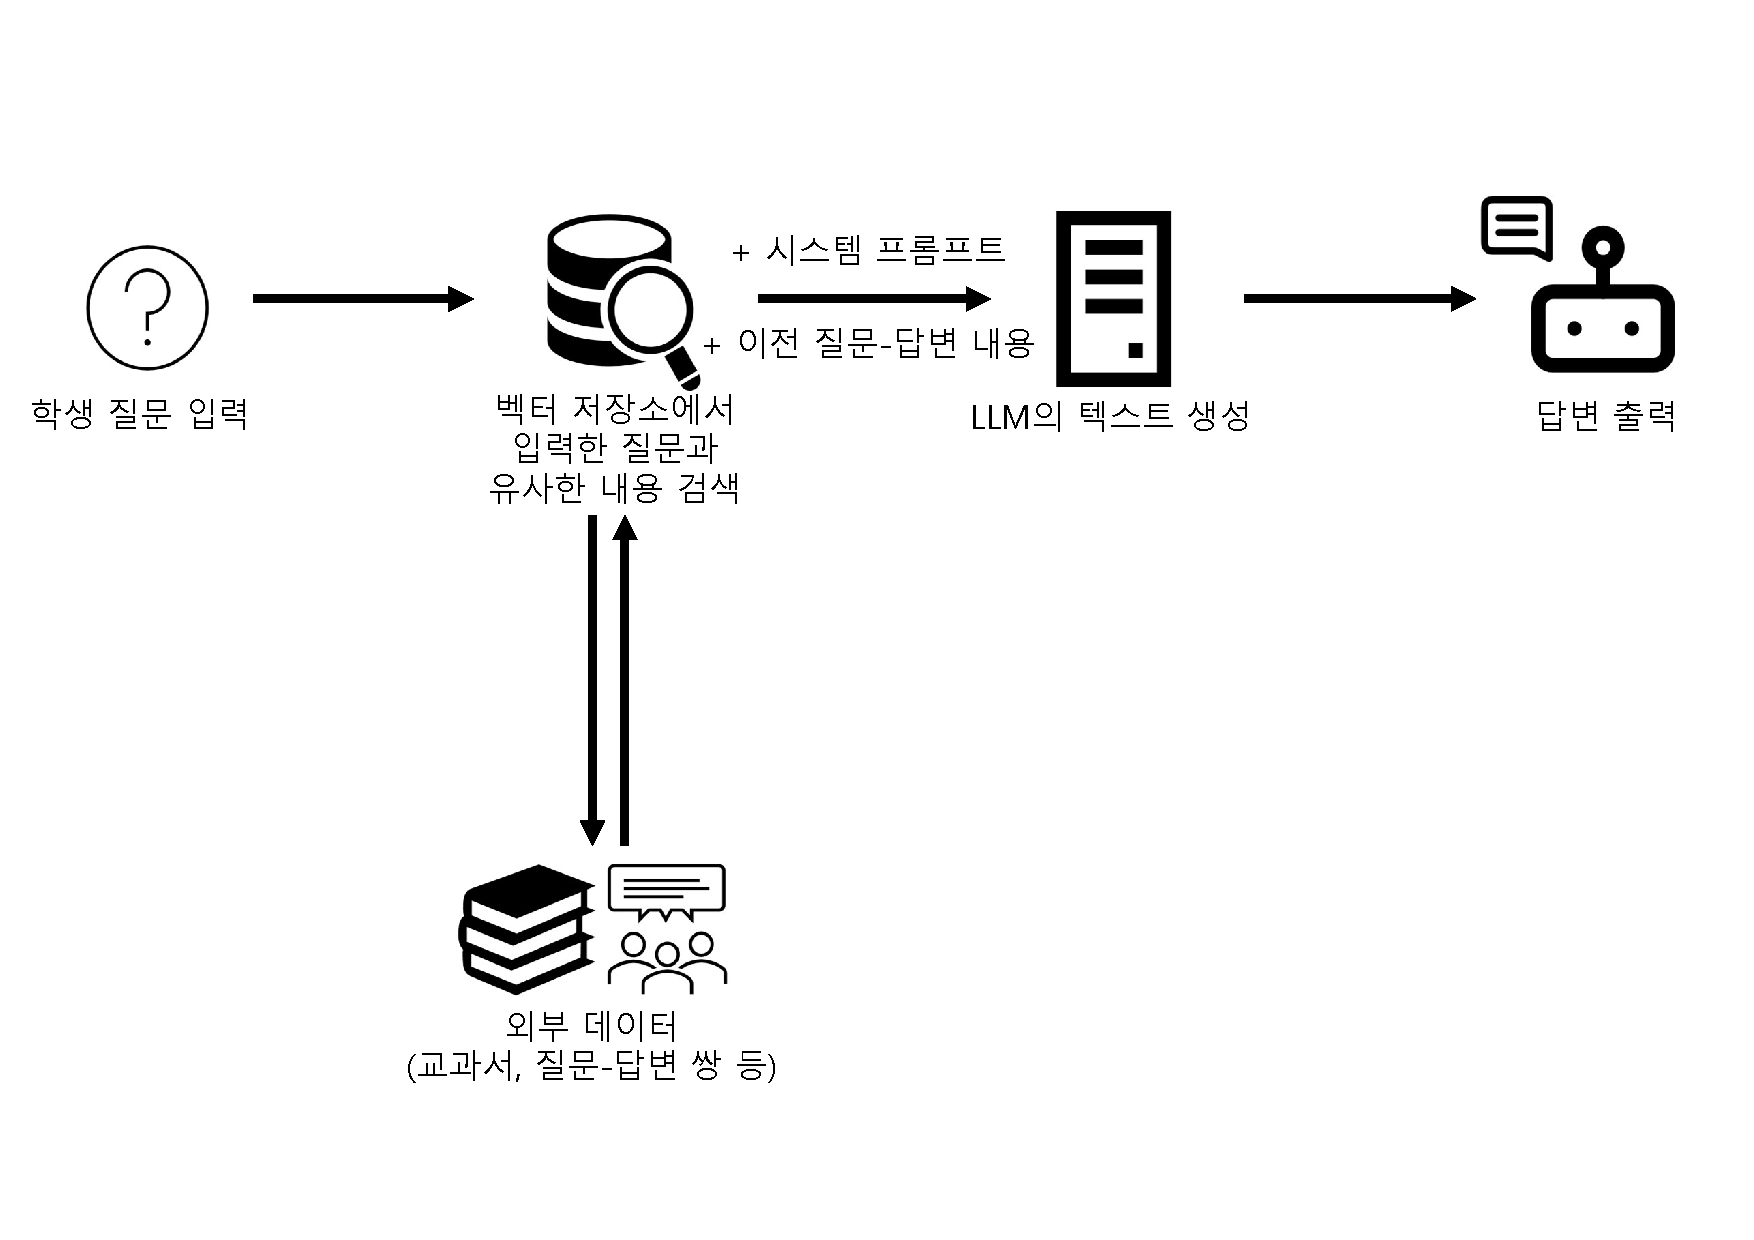
\includegraphics[width=12cm]{pdfs/method-RAG.pdf}
    \caption{LLM에 RAG를 적용하여 답변을 생성하는 과정}
    \label{method-RAG}
\end{figure}

/figs 폴더에도 그림을 넣어서 사용했습니다. 이 디렉토리는 비워두겠습니다.

\subsubsection{subsubsection도 넣을 수 있어요}

...

\subsubsection{subsubsection도 넣을 수 있어요}

...

\subsubsection{subsubsection도 넣을 수 있어요}

\cite{min2024}\가 ... 처럼 쓰면 이/가도 자동으로 바뀝니다.

\subsubsection{subsubsection도 넣을 수 있어요}

강조용 글꼴 변화는 texttt를 사용하세요.

PDF 파일을 불러온 내용을 내용을 일반적인 문장으로 만들기 위해 \texttt{$\backslash$x}로 시작하는 ... 부분을 제외하고자 \texttt{진도체크, 보고서 작성하기, 도움 영상, 발표하기, 고르시오, ㄱ, ㄴ, ㄷ, 만들어 보자, 평가하기} 등 총 50가지 정도의 문구가 있는 문장을 삭제했다.

...

\subsubsection{시스템 프롬프트 구성}

컴퓨터 코드 삽입 예시

2024년 9월에 최종적으로 수정한 시스템 프롬프트는 \Cref{gen-prompt-new}\와 같다.

\begin{figure}[h!]
    \begin{lstlisting}
        template = '''[BOS]system
        당신은 고등학교 과학 선생님입니다. 학생들의 질문에 200 단어 이내의 한국어로만 답변해야 합니다.
        중요: 다음 규칙을 반드시 따르세요.
        1. 출력 관련 지시사항:
        (1) Markdown 을 써서 가독성을 높이세요.
        (2) 모든 수식은 무조건 이중 '$' 기호로 감싸서 출력해야만 합니다. 예: $$ 3 mol $$
        (3) http 나 https 로 시작하는 URL 은 무조건 plain text 로 표현하세요 !
        2. 학생이 입력한 질문이 " 안녕하세요 ? ", " 안녕 ? ", " 고마워 ", " 감사합니다 " 와 같은 인사나 감사 표현이라면:
        (1) HISTORY 와 CONTEXT 를 완전히 무시하세요.
        (2) 오직 해당 인사에 대해서만 간단히 응답하세요.
        (3) 이 경우, ' 생각 '과 ' 답변 ' 구조를 사용하지 마세요.
        3. 그밖의 모든 질문에 대해서는:
        (1) ' 생각 '과 ' 답변 ' 두 부분으로 나누어 응답하세요.
        (2) CONTEXT 와 HISTORY 로부터 답변할 수 있는 경우 가장 우선적으로 참조하여 답변하세요.
        (3) 관련 정보가 없는 경우, 자체 지식을 사용하세요.
        (4) 답변할 수 없는 경우 " 죄송합니다. 제가 알지 못하는 내용입니다. "라고 말하세요.
        (5) 고등학교 1 학년 학생이 이해할 수 있는 적절한 용어를 사용하세요.
        HISTORY: {history}
        CONTEXT: {context}
        HUMAN: {question}
        [|endofturn|]
        [BOS]human
        {question}
        [|endofturn|]
        [BOS]assistant
        
        [|endofturn|]'''
    \end{lstlisting}
    \caption{교사와 학생의 평가를 반영하여 개선한 시스템 프롬프트}
    \label{gen-prompt-new}
\end{figure}

표 작성 예시

표와 그림은 모두 Cref로 언급하면 자동으로 표와 그림을 나누어 번호가 매겨집니다.

두 가지 학교 맞춤형 과학 질문-답변 챗봇의 사용 기록 및 사용자 평가 내용의 개요는 \Cref{methods-comparison-verdict}\와 같다.

\begin{table}
    \centering
    \caption{두 가지 학교 맞춤형 과학 질문-답변 챗봇의 사용 기록 및 사용자 평가 내용의 개요}
    \resizebox{0.9\textwidth}{!}{%
    \begin{tabular}{ccc}
        \hline
        범주 & 선행연구 1 & 선행연구 2 \\
        \hline
        자료 수집 기간과 학생의 챗봇 활용 관련 자료 수집 방법 & O & O \\
        학생이 주로 챗봇을 활용한 시간과 사용한 기기 & O & O \\
        학생의 질문 주제 분류 & O & O \\
        학생의 챗봇 사용상 나타나는 특징 & O & O \\
        학생의 설문조사 응답 결과 & X & O \\
        \hline
    \end{tabular}
    }
    \label{methods-comparison-verdict}
\end{table}

복잡한 표 작성 예시 1

multicolumn, multirow\를 적극적으로 활용하세요. 오류가 가장 적게 납니다.

\begin{table}[h!]
    \centering
    \caption{LLM별 RAG 적용 실험 조건}
    \begin{tabular}{ll}
    \hline
    \multicolumn{1}{c}{\textbf{오픈소스 LLM}} & \multicolumn{1}{c}{\textbf{실험 조건}} \\ \hline
    LG EXAONE 3.0 7.8B &
    \begin{tabular}{l}
    1. 교사용 교과서와 질문-답변 쌍 모두 활용 \\
    2. 교사용 교과서만 활용 \\
    3. 질문-답변 쌍만 활용 \\
    4. RAG 적용 안 함
    \end{tabular} \\ \hline
    Google Gemma 2 9B & 
    \begin{tabular}{l}
    1. 교사용 교과서와 질문-답변 쌍 모두 활용 \\
    2. 교사용 교과서만 활용 \\
    3. 질문-답변 쌍만 활용 \\
    4. RAG 적용 안 함
    \end{tabular} \\
    \hline
    \end{tabular}
    \label{method-crossexperiment_by_llm}
\end{table}


복잡한 표 작성 예시 2

학생 질문을 주제별로 분류한 결과는 \Cref{doc2vec-table1}\과 같다.

\begin{table}[h!]
    \centering
    \caption{학생 질문을 주제별로 분류한 결과\citep{min2022}}
    \label{doc2vec-table1}
    \begin{tabular}{ccc}
    \hline
    {\textbf{대분류}} & {\textbf{소분류}} & \textbf{개수 (비율)} \\ \hline
    \multirow{10}{*}{교과 (1,168개, 52.4\%)} & 중3 교과내용 관련 & 868 (38.9\%) \\ \cline{2-3} 
     & 지필평가 & 103 (4.6\%) \\ \cline{2-3} 
     & 수행평가 & 72 (3.2\%) \\ \cline{2-3} 
     & 시험범위 & 33 (1.5\%) \\ \cline{2-3} 
     & 교육과정 & 25 (1.1\%) \\ \cline{2-3} 
     & 중1 교과내용 관련 & 20 (0.9\%) \\ \cline{2-3} 
     & 중2 교과내용 관련 & 20 (0.9\%) \\ \cline{2-3} 
     & 서술형 시험 & 16 (0.7\%) \\ \cline{2-3} 
     & 수업 & 7 (0.3\%) \\ \cline{2-3} 
     & 과제 & 4 (0.2\%) \\ \hline
    \multirow{7}{*}{교과 외 (1,062개, 47.6\%)} & 잡담 & 503 (22.6\%) \\ \cline{2-3} 
     & 챗봇 & 187 (8.4\%) \\ \cline{2-3} 
     & 상담 & 105 (4.7\%) \\ \cline{2-3} 
     & 교사 & 96 (4.3\%) \\ \cline{2-3} 
     & 타 과목 & 96 (4.3\%) \\ \cline{2-3} 
     & 인사 & 42 (1.9\%) \\ \cline{2-3} 
     & 욕설 & 33 (1.5\%) \\ \hline
    \multicolumn{2}{c}{\textbf{합계}} & 2,230 (100\%) \\ \hline
    \end{tabular}
\end{table}

\chapter{연구 결과}\label{results}
\section{section 제목}

\subsection{subsection 제목}

\subsubsection{subsubsection 제목}

\paragraph{subsubsection 제목}

subsubsection 아래에 paragraph로 나누어서 작성할 수도 있습니다

...

\paragraph{paragraph 제목}

...

\paragraph{paragraph 제목}

...

\chapter{결론 및 논의}
\section{결론 및 논의}

...

\paragraph*{학위논문은 호흡이 길어서 paragraph*로 나누어서 가독성을 높였습니다}

*을 붙이면 차례에 나타나지 않습니다.

\paragraph*{paragraph 제목}

...

\paragraph*{paragraph 제목}

...

\paragraph*{연구의 의의}

...

\section{연구의 한계}

...

\section{향후 연구 방향}

...

마지막으로, 참고문헌은 references.bib에서 본문에 쓰지 않은 것을 굳이 지우지 않아도 됩니다. biber가 알아서 본문에 나온 것만 참고문헌을 작성합니다. 한국어 논문을 참고문헌으로 쓸 경우 refrences.bib에 keywords={kobib}를 넣어주기만 하면 영어 논문과 한글 논문을 구분하여 참고문헌이 자동으로 작성됩니다.

%%%%%%%%%%%%%%%%%%%%%%%%%%%%%%%%% Bibliography %%%%%%%%%%%%%%%%%%%%%%%%%%%%%%%%%%%
\clearpage
\printbibliography[title={참고문헌}]
%\addcontentsline{toc}{chapter}{참고문헌}
%\bibliographystyle{aa_url}
%\setstretch{1.0}  % ← of course you can change this as you wish, too.
%\bibliography{references.bib}
%%%%%%%%%%%%%%%%%%%%%%%%%%%%%%%%%%%%%%%%%%%%%%%%%%%%%%%%%%%%%%%%%%

\appendix % 부록은 연구에 맞추어 수정하세요
\chapter{연구에서 사용했던 약어 목록}
\begin{sortedlist}
    % 아래 목록을 자동으로 가나다순 정렬합니다.
    \sortitem{API: Application Programming Interface}
    \sortitem{LLM: Large Language Model}
    \sortitem{sLLM: Small Large Language Model}
    \sortitem{SLM: Small Language Model}
    \sortitem{LDA: Latent Dirichlet Allocation}
    \sortitem{LTS: Long Term Support}
    \sortitem{RAG: Retrieval-Augmented Generation}
    \sortitem{NLP: Natural Language Processing}
    \sortitem{BERT: Bidirectional Encoder Representations from Transformers}
    \sortitem{RoBERTa: Robustly optimized BERT pretraining approach}
    \sortitem{GPT: Generative Pre-trained Transformer}
    \sortitem{GPU: Graphics Processing Unit}
    \sortitem{NPU: Neural Processing Unit}
    \sortitem{IRQA: Information Retrieval-based Question Answering}
    \sortitem{UUID: Universally Unique Identifier}
    \sortitem{VRAM: Video Random Access Memory}
    \sortitem{MMR: Maximal Marginal Relevance}
    \sortitem{BOS: Beginning of Sentence}
    \sortitem{WSGI: Web Server Gateway Interface}
    \sortitem{ASGI: Asynchronous Server Gateway Interface}
\end{sortedlist}

\chapter{IRB 결과 통보서와 연구 참여자 모집 문건, 설문지}
IRB 결과 통보서와 연구 참여자 모집 문건, 설문지를 첨부하였다.

교사와 학생으로부터 설문지 응답을 받기 위해 연구 참여자 모집 문건과 설문지와 관련하여 IRB의 승인을 받았다.

% PDF를 통째로 넣을 수 있습니다. Microsoft PDF Printer로 만든 PDF 파일과 호환성이 높습니다.
% 주석을 해제하여 사용하세요.

%\includepdf[pages=-,pagecommand={},width=\textwidth]{pdfs/gen1.pdf}
%\includepdf[pages=-,pagecommand={},width=\textwidth]{pdfs/gen2.pdf}

%%%%%%%%%%%%%%%%%%%%%%%%%%%% 영문초록 %%%%%%%%%%%%%%%%%%%%%%%%%%%%%%%
\setstretch{2.0} % 영문초록의 줄간격
\chapter*{Abstract}\addcontentsline{toc}{chapter}{Abstract}%\setcounter{page}{3}

\begin{center}
  \begin{huge}
    INPUT YOUR TITLE IN ENGLISH
  \end{huge}
\end{center}

\begin{flushright}
  \begin{large}
    Gildong Hong

    Physics Education
    
    The Graduate School
    
    Seoul National University    
  \end{large}
\end{flushright}

\quad Recent advances in Large Language Models (LLMs) have enhanced the potential for developing educational chatbots. 

\quad ...

\quad ...

~\\
\hangindent=2em
\hangafter=2
\textbf{Keywords}: Keyword1, Keyword2, Keyword3, Keyword4, Keyword5, Keyword6

~\\
\noindent \textbf{Student Number}: 2020-30000

%%%%%%%%%%%%%%%%%%%%%%%%%%%%%%%%%%%%%%%%%%%%%%%%%%%%%%%%%%%%%%%%%%

%\chapter*{Acknowledgement}\\
%\twocolumn

% 감사의 말은 꼭 필요하지는 않아서 생략 %%%%%%%%%%%%%%%%%%%%%%%%%%%%%%
%\strangechapter{Ack}{Acknowledgement}\addcontentsline{toc}{chapter}{Acknowledgement}
%\small
%\footnotesize
%\setstretch{1.1}
%\setlength{\parskip}{0.3em}
%\input{chaps/acknowledgement}
%%%%%%%%%%%%%%%%%%%%%%%%%%%%%%%%%%%%%%%%%%%%%%%%%%%%%%%%%%%%%%%%%%%

\end{document}